\section{Trực quan hóa dữ liệu với Power BI}

\subsection{Mục tiêu Dashboard}
Sau khi xây dựng Data Warehouse trên SQL Server, nhóm kết nối Power BI trực tiếp đến schema \texttt{dw}. Dashboard được thiết kế để trả lời ba nhóm câu hỏi nghiệp vụ:
\begin{itemize}
    \item Quy mô danh mục khoản vay hiện tại là bao nhiêu?
    \item Nhóm khách hàng/khoản vay nào có tỷ lệ nợ xấu cao?
    \item Các đặc trưng như thu nhập, hạng tín dụng, kỳ hạn vay và tình trạng nhà ở ảnh hưởng đến rủi ro như thế nào?
\end{itemize}

Để thao tác Power BI đơn giản hơn, script SQL tạo thêm view \texttt{dw.vw\_Loan\_Dashboard}. View này nối sẵn \texttt{Fact\_Loan}, \texttt{Dim\_Borrower} và \texttt{Dim\_Loan\_Info}; vì vậy khi dựng dashboard, nhóm có thể kéo thả field từ một view duy nhất.

\subsection{Chuẩn bị dữ liệu trong Power BI}
\subsubsection{Kết nối dữ liệu}
Các bước kết nối:
\begin{enumerate}
    \item Chọn \textbf{Get Data} $\rightarrow$ \textbf{SQL Server}.
    \item Nhập server, ví dụ \texttt{localhost}, và database \texttt{Loan\_Approval\_DW}.
    \item Chọn view \texttt{dw.vw\_Loan\_Dashboard}. Nếu muốn trình bày mô hình sao, có thể chọn thêm \texttt{dw.Fact\_Loan}, \texttt{dw.Dim\_Borrower}, \texttt{dw.Dim\_Loan\_Info}.
    \item Chọn \textbf{Import} để dashboard chạy nhanh trên tập mẫu 100.000 dòng.
\end{enumerate}

\subsubsection{Các Measure DAX}
Nhóm tạo các measure chính sau trong Power BI:

\begin{lstlisting}[language=SQL, caption=Measure DAX sử dụng trong Dashboard]
Total Loans = COUNT('vw_Loan_Dashboard'[Fact_ID])

Bad Loans =
CALCULATE(
    COUNT('vw_Loan_Dashboard'[Fact_ID]),
    'vw_Loan_Dashboard'[loan_status_bin] = 1
)

Good Loans =
CALCULATE(
    COUNT('vw_Loan_Dashboard'[Fact_ID]),
    'vw_Loan_Dashboard'[loan_status_bin] = 0
)

Bad Loan Rate = DIVIDE([Bad Loans], [Bad Loans] + [Good Loans])

Average Loan Amount = AVERAGE('vw_Loan_Dashboard'[loan_amnt])

Average Interest Rate = AVERAGE('vw_Loan_Dashboard'[int_rate])
\end{lstlisting}

\textit{Lưu ý:} \texttt{Bad Loan Rate} không chia cho toàn bộ \texttt{Total Loans}, vì một số trạng thái như \textit{In Grace Period} có \texttt{loan\_status\_bin} rỗng. Công thức chỉ tính trên các hồ sơ đã có nhãn tốt/xấu rõ ràng.

\subsection{Thiết kế các biểu đồ chính}
\subsubsection{KPI Cards}
Phần đầu dashboard nên dùng các \textbf{Card Visuals} để hiển thị nhanh tình hình tổng quan:
\begin{itemize}
    \item \textbf{Total Loans:} tổng số khoản vay sau khi load vào fact.
    \item \textbf{Bad Loans:} số khoản vay rủi ro/nợ xấu.
    \item \textbf{Bad Loan Rate:} tỷ lệ nợ xấu trên các hồ sơ đã có nhãn tốt/xấu.
    \item \textbf{Average Loan Amount:} số tiền vay trung bình.
    \item \textbf{Average Interest Rate:} lãi suất trung bình.
\end{itemize}

\textbf{Cách làm trong Power BI:} chọn visual \textit{Card}, kéo từng measure vào ô \textit{Fields}. Với \texttt{Bad Loan Rate}, định dạng kiểu Percentage và làm tròn 1--2 chữ số thập phân.

\subsubsection{Biểu đồ 1: Phân bổ trạng thái khoản vay}
\begin{itemize}
    \item \textbf{Visual:} Clustered Bar Chart hoặc Donut Chart.
    \item \textbf{Axis/Legend:} \texttt{loan\_status\_raw}.
    \item \textbf{Values:} \texttt{Total Loans}.
\end{itemize}

\textbf{Ý nghĩa:} Biểu đồ này cho biết cơ cấu trạng thái khoản vay sau khi loại \textit{Current}. Nếu nhóm \textit{Fully Paid} chiếm đa số, danh mục có nhiều hồ sơ đã hoàn tất tốt. Các nhóm \textit{Charged Off}, \textit{Default} và \textit{Late} là vùng cần chú ý vì phản ánh rủi ro tín dụng.

\subsubsection{Biểu đồ 2: Histogram thu nhập khách hàng}
Theo yêu cầu đề bài, dashboard cần có biểu đồ histogram. Trong dự án này, nhóm tạo histogram bằng cột \texttt{income\_bin} đã được phân thùng trong SQL.

\begin{itemize}
    \item \textbf{Visual:} Clustered Column Chart.
    \item \textbf{X-axis:} \texttt{income\_bin}.
    \item \textbf{Y-axis:} \texttt{Total Loans}.
    \item \textbf{Format:} giảm \textit{Inner Padding} để các cột đứng gần nhau hơn.
\end{itemize}

\textbf{Cách kéo đúng:} không kéo \texttt{Fact\_ID} vào trục Y dưới dạng giá trị thô. Phải dùng measure \texttt{Total Loans = COUNT(Fact\_ID)} cho Y-axis, còn \texttt{income\_bin} nằm ở X-axis. Nếu kéo ngược lại, Power BI sẽ tạo một khối biểu đồ sai và không thể hiện được phân phối tần suất.

\textbf{Ý nghĩa:} Kết quả trên tập \texttt{living\_sample\_100k.csv} cho thấy nhóm \textit{Medium Income (50k--100k)} chiếm nhiều nhất, tiếp theo là \textit{Low Income (<50k)} và \textit{High Income (>100k)}. Điều này cho thấy danh mục vay tập trung chủ yếu ở nhóm thu nhập trung bình.

\begin{figure}[H]
    \centering
    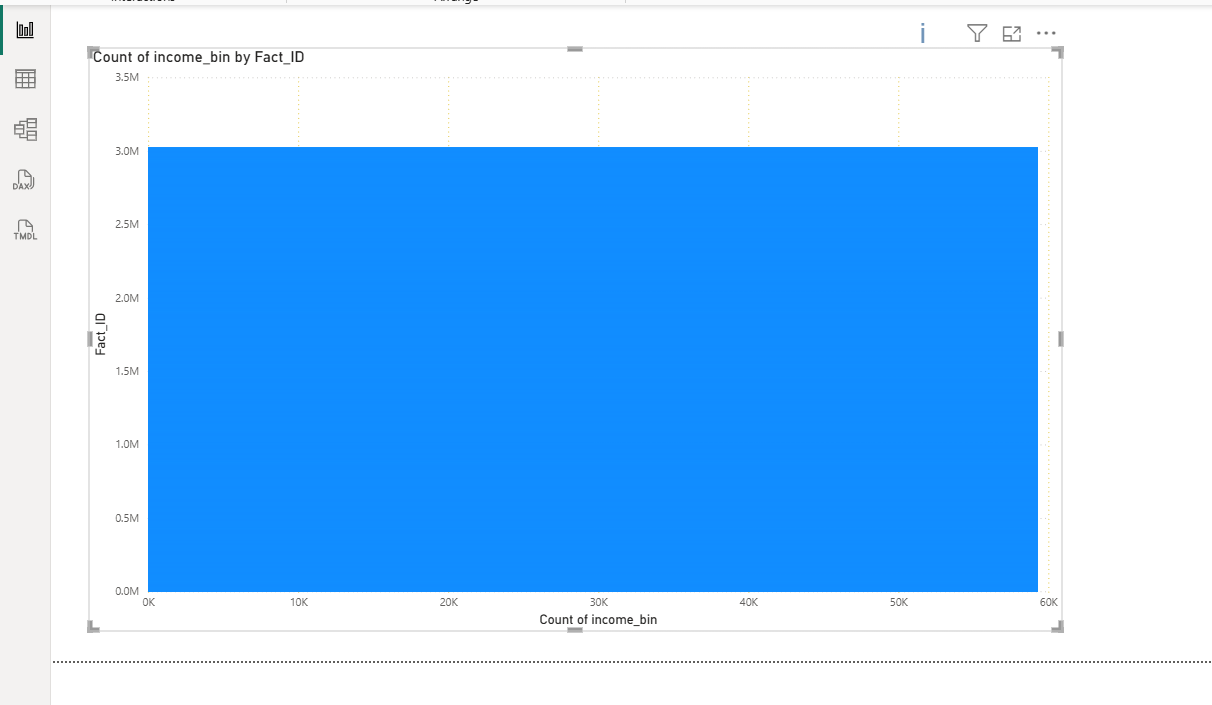
\includegraphics[width=0.75\textwidth]{images/Screenshot 2026-05-14 084744.png}
    \caption{Minh họa biểu đồ Histogram phân bổ khách hàng theo nhóm thu nhập}
    \label{fig:histogram_income}
\end{figure}

\subsubsection{Biểu đồ 3: Tỷ lệ nợ xấu theo hạng tín dụng}
\begin{itemize}
    \item \textbf{Visual:} Line and Clustered Column Chart hoặc Clustered Column Chart.
    \item \textbf{X-axis:} \texttt{grade}.
    \item \textbf{Column values:} \texttt{Total Loans}.
    \item \textbf{Line values:} \texttt{Bad Loan Rate}.
\end{itemize}

\textbf{Ý nghĩa:} Hạng tín dụng càng thấp thì rủi ro càng cao. Trên tập mẫu, tỷ lệ nợ xấu tăng dần từ nhóm A đến G: hạng A khoảng 6,7\%, hạng C khoảng 24,3\%, hạng E khoảng 39,4\% và hạng G hơn 51\%. Đây là insight quan trọng, chứng minh biến \texttt{grade} có ý nghĩa mạnh trong đánh giá rủi ro.

\subsubsection{Biểu đồ 4: Tỷ lệ nợ xấu theo kỳ hạn vay}
\begin{itemize}
    \item \textbf{Visual:} Clustered Column Chart.
    \item \textbf{X-axis:} \texttt{term}.
    \item \textbf{Y-axis:} \texttt{Bad Loan Rate}.
    \item \textbf{Tooltip:} \texttt{Total Loans}, \texttt{Average Interest Rate}.
\end{itemize}

\textbf{Ý nghĩa:} Khoản vay 60 tháng có tỷ lệ nợ xấu cao hơn khoản vay 36 tháng. Trên tập mẫu, nhóm 36 tháng có tỷ lệ nợ xấu khoảng 17,3\%, trong khi nhóm 60 tháng khoảng 34,0\%. Điều này phù hợp với nghiệp vụ tín dụng: kỳ hạn càng dài, rủi ro biến động thu nhập và khả năng trả nợ càng lớn.

\subsubsection{Biểu đồ 5: Tỷ lệ nợ xấu theo nhóm thu nhập}
\begin{itemize}
    \item \textbf{Visual:} Clustered Column Chart.
    \item \textbf{X-axis:} \texttt{income\_bin}.
    \item \textbf{Y-axis:} \texttt{Bad Loan Rate}.
\end{itemize}

\textbf{Ý nghĩa:} Nhóm \textit{Low Income} có tỷ lệ nợ xấu cao nhất, khoảng 24,0\%; nhóm \textit{Medium Income} khoảng 21,3\%; nhóm \textit{High Income} khoảng 17,6\%. Insight này cho thấy thu nhập thấp không chỉ làm giảm năng lực trả nợ mà còn là tín hiệu quan trọng trong phân tích rủi ro.

\subsubsection{Bộ lọc tương tác}
Dashboard nên có các slicer sau:
\begin{itemize}
    \item \texttt{grade}: lọc theo hạng tín dụng.
    \item \texttt{term}: lọc theo kỳ hạn vay.
    \item \texttt{home\_ownership}: lọc theo tình trạng nhà ở.
    \item \texttt{verification\_status}: lọc theo trạng thái xác minh thu nhập.
\end{itemize}

Các slicer giúp người dùng phân tích cùng một chỉ số dưới nhiều góc nhìn. Ví dụ, khi chọn riêng kỳ hạn 60 tháng, dashboard sẽ cho thấy nhóm nào có tỷ lệ nợ xấu cao hơn trong phân khúc vay dài hạn.

\subsection{Nhận xét tổng hợp}
Dashboard Power BI cho thấy ba insight chính:
\begin{enumerate}
    \item \textbf{Hạng tín dụng là biến phân tách rủi ro mạnh:} tỷ lệ nợ xấu tăng rõ rệt từ grade A đến G.
    \item \textbf{Kỳ hạn vay dài làm tăng rủi ro:} khoản vay 60 tháng có tỷ lệ nợ xấu gần gấp đôi khoản vay 36 tháng.
    \item \textbf{Thu nhập có liên hệ với khả năng trả nợ:} nhóm thu nhập thấp có tỷ lệ nợ xấu cao hơn nhóm thu nhập cao.
\end{enumerate}

Những insight này giúp bộ phận tín dụng điều chỉnh chính sách phê duyệt, chẳng hạn kiểm soát chặt hơn với khách hàng có grade thấp, kỳ hạn dài và thu nhập thấp.
